\documentclass[11pt]{article}
\usepackage[english]{babel}
\usepackage{geometry}
\usepackage{amsmath}
\usepackage{amsthm}
\usepackage{graphicx}
\usepackage[utf8]{inputenc}

%%%%%%%% MARGIN
\geometry{verbose, letterpaper, tmargin=3cm,
  bmargin=3cm,lmargin=2.5cm,rmargin=2.5cm}

%%%%%%%% PARAGRAPH SETTINGS
% https://tex.stackexchange.com/questions/27802/set-noindent-for-entire-file
\setlength\parindent{0pt}

% https://tex.stackexchange.com/questions/49188/how-to-insert-vertical-space-between-paragraphs
\setlength{\parskip}{5pt}

%%%%%%%% SUB-FIGURE PACKAGE
\usepackage{subcaption}

%%%%%%%% HYPERREF PACKAGE
\usepackage{hyperref}
\hypersetup{linkcolor=blue}
\hypersetup{citecolor=blue}
\hypersetup{urlcolor=blue}
\hypersetup{colorlinks=true}

%%%%%%%% DEFINITION AND THEOREM DEFINITIONS
\theoremstyle{definition}
\newtheorem{definition}{Definition}[section]

\theoremstyle{remark}
\newtheorem{remark}{Remark}

\theoremstyle{remark}
\newtheorem{question}{Question}

\newtheorem{theorem}{Theorem}[section]

%%%%%%%% MULTI-COLUMNS PACKAGE
\usepackage{multicol}

%%%%%%%% BIB-LATEX STUFF
\usepackage[style=numeric,
            bibstyle=numeric,
            citestyle=numeric,
            hyperref=true,
            backend=biber]{biblatex}
\addbibresource{ref.bib} %Put relative path to ref

%%%%%%%% PERSONAL COMMANDS
\usepackage{amssymb}

%%%% Important sets
\renewcommand{\O}{\mathbb{O}}
\newcommand{\N}{\mathbb{N}}
\newcommand{\Z}{{\mathbb{Z}}}
\newcommand{\Q}{{\mathbb{Q}}}
\newcommand{\R}{{\mathbb{R}}}

%%%% Usual operations
\newcommand{\pow}[2]{#1^{#2}}
\newcommand{\expp}[1]{e^{#1}}
\newcommand{\fst}{\mathrm{fst}}
\newcommand{\snd}{\mathrm{snd}}

%%%% Lambda Calculus
\newcommand{\dneq}{\,\, \# \,\,}
\renewcommand{\S}{\pmb{\mathrm{S}}}
\newcommand{\I}{\pmb{\mathrm{I}}}
\newcommand{\K}{\pmb{\mathrm{K}}}
\newcommand{\ch}[1]{\ulcorner #1 \urcorner}

%%%% Ordinal Lambda Calculus
\newcommand{\ordAlph}{\Sigma_{\text{Ord}}}
\newcommand{\termOrd}{\text{Term}_\text{Ord}}
\newcommand{\fl}{\mathrm{fl}}
\newcommand{\sk}{\mathrm{sk}}

%% Superscript to the left
% https://latex.org/forum/viewtopic.php?t=455
\usepackage{tensor}
\newcommand{\app}[3]{\tensor*[^{#1}]{\left(#2, #3\right)}{}}

%%%% Make optional parameter
% https://tex.stackexchange.com/questions/217757/special-behavior-if-optional-argument-is-not-passed
\usepackage{xparse}

%%%% Statistics
\NewDocumentCommand{\E}{o m}{
  \IfNoValueTF{#1}
  {\mathbb{E}\left[#2\right]}
  {\mathbb{E}^{#1}\left[ #2\right]}
}
\NewDocumentCommand{\V}{o m}{
  \IfNoValueTF{#1}
  {\mathrm{Var}\left[#2\right]}
  {\mathrm{Var}^{#1}\left[ #2\right]}
}
\RenewDocumentCommand{\P}{o o m}{
  \IfNoValueTF{#1}
  {\IfNoValueTF{#2}
    {\mathrm{P}\left(#3\right)}
    {\mathrm{P}^{#2}\left(#3\right)}}
  {\IfNoValueTF{#2}
    {\mathrm{P}_{#1}\left(#3\right)}
    {\mathrm{P}_{#1}^{#2} \left(#3\right)}}
}

%%%% Lambda Calculus
\NewDocumentCommand{\cx}{o}{
  \IfNoValueTF{#1}
  {\left[\quad\right]}
  {\left[\, #1 \,\right]}
}

%%%% Create absolute value function
% https://tex.stackexchange.com/questions/43008/absolute-value-symbols
\usepackage{mathtools}
\DeclarePairedDelimiter\abs{\lvert}{\rvert}%
\DeclarePairedDelimiter\norm{\lVert}{\rVert}%
\makeatletter
\let\oldabs\abs
\def\abs{\@ifstar{\oldabs}{\oldabs*}}
%
\let\oldnorm\norm
\def\norm{\@ifstar{\oldnorm}{\oldnorm*}}
\makeatother

%%%%%%%% LOGIC TREES
\usepackage{prftree}

%%%%%%%% SPLIT EQUATIONS
% https://tex.stackexchange.com/questions/51682/is-it-possible-to-pagebreak-aligned-equations
\allowdisplaybreaks

%%%%%%%% FLOAT SPECIFIER
% https://www.overleaf.com/learn/latex/Errors/LaTeX_Error:_Unknown_float_option_%60H%27
\usepackage{float}

%%%%%%%% TO USE SHORT COMMANDS FOR VECTOR LINES
\usepackage{esvect}

%%%%%%%% ENUMERATE LABEL
% https://www.latex-tutorial.com/tutorials/lists/
\usepackage{enumitem}

%%%%%%%% DIFFERENT FONTS FOR MATH
\usepackage{mathrsfs}

%%%%%%%% CODE RENDERING !!! UNCOMMENT IF NEEDED !!!
% Compile with flag -shell-escape
%\usepackage{minted}

%%%%%%%% START DOCUMENT
\title{Final Work}
\author{Juan Sebasti\'an C\'ardenas-Rodríguez \\
  \scalebox{0.7}{Mathematical Engineering, Universidad EAFIT}}
\date{\today}


\begin{document}
\maketitle

\section{Option Pricing}
\subsection{Question 2}
The free risk rate of Facebook was taken from \href{https://bit.ly/30yrDY4}{Guru
  Focus}. The free risk rate was extracted from the website on the 2nd of June
of 2020. The value for this rate is $r = 0.65\%$.

On the other hand, the volatility was estimated by using the Maximum Likelihood
methodology. Let $y_{i}$ for $i = 1, 2, \ldots, n$ be the prices of the stock.
Then, in the first place, the returns $\omega_{i}$ are calculated by:
\begin{equation*}
  \omega_{i} = \frac{y_{i + 1} - y_{i}}{y_{i}}
\end{equation*}
It is important to remark that the amount of returns is one less than the data.
The time series for the returns can be seen in Figure \ref{fig:rtjs}. Finally,
the volatility $\sigma$ is estimated by the following equation:
\begin{equation*}
  \sigma = \frac{1}{(n - 2) \Delta t} \sum_{i = 1}^{n - 1}\left(\omega_{i} -
    \frac{1}{n - 1}\sum_{i=1}^{n - 1} \omega_{i}\right)^{2}
\end{equation*}
The result for this estimation is $\sigma = 0.025$.

\begin{figure}[ht]
  \centering
  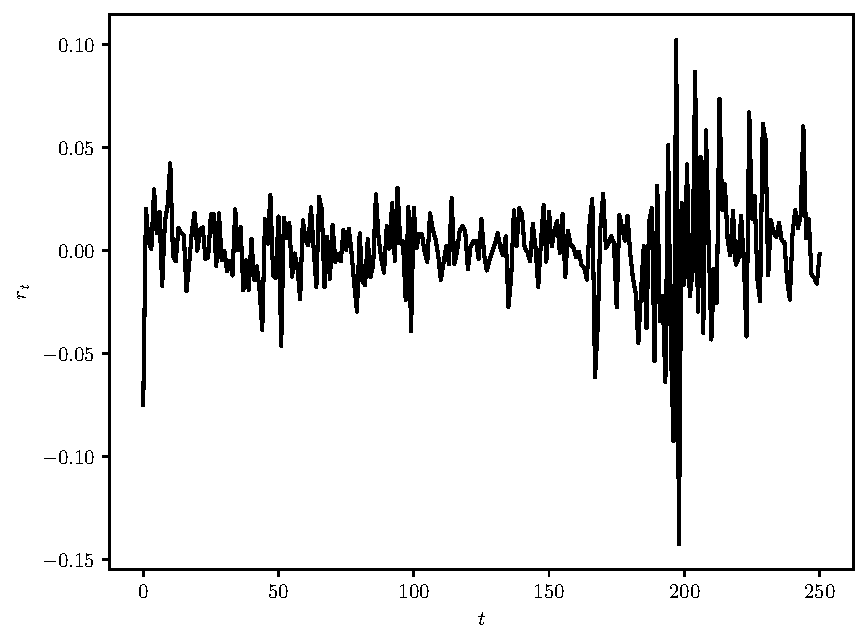
\includegraphics[scale=.7]{../plts/returns_js}
  \caption{Time series for returns used for ML methology.}
  \label{fig:rtjs}
\end{figure}

\subsection{Question 3}
The stock pricing was realized with Black-Scholes, Monte Carlo simulation,
binomial trees, and finite differences. The pricing obtained with Black-Scholes
is considered to be the exact pricing for the Facebook stock.

For each method, a time series for the returns are calculated. Differently to
the previous question, the returns are calculated by:
\begin{equation*}
  \omega_{i} = \log\left(\frac{y_{i + 1}}{y_{i}}\right)
\end{equation*}
with $y_{i}$ are the prices for the Facebook stock. Furthermore, it is important
to notice that this returns also have one less data than the stock prices.

\textcite{black1973} created a methodology to correctly price a European call
option. Nowadays, this methodology is known as the Black-Scholes method. Let
$\sigma$ be the volatility of the stock, $T$ the time for that option. Then, two
quantiles are calculated by:
\begin{equation*}
  d_{1} = \frac{1}{\sigma \sqrt{T}} \left(\log\left(\frac{S_{0}}{K}\right)
    + \left(r + \frac{1}{2}\sigma^{2}\right) T\right), \qquad d_{2} = d_{1} - \sigma \sqrt{T}
\end{equation*}
Lastly, using these quantiles the pricing for the option $f$ is calculated as follows:
\begin{equation*}
  f = S_{0} F(d_{1}) - K \expp{-rT} F(d_{2})
\end{equation*}

with $F(\cdot)$ the continuous distribution function for a standard normal
distribution.

The second method used was a Monte Carlo simulation approach. This approach was
created by \textcite{boyle1977}. The Monte Carlo simulation method first
simulates the selected differential equation with $M$ trajectories. In the case
of the returns, the process is a Geometric Brownian Motion, which is discretized
as:
\begin{equation*}
  S_{t + \Delta t} = S_{t}\expp{\left(r - \frac{\sigma^{2}}{2}\right) + \sigma \Delta B_{t}}
\end{equation*}
Then, the payoff is calculated by:
\begin{equation*}
  p_{i} = \max(S_{i,T} - K, 0)
\end{equation*}
Consequently, then the $f_{\text{call}}$ is calculated by the following
equation:
\begin{equation*}
  f_{\text{call}} = e^{-rT} \E{p}
\end{equation*}
This process is repeated $W$ times, saving the results of each simulation.
Finally, the mean of all the $f_{\text{call}}$ is calculated to estimate the
pricing of the option.

The Binomial Tree method was created by \textcite{cox1979}. This method consists
of defining a barrier for a binomial tree and, then calculating the value for
the root by regressing. An example of a binomial tree can be seen in Figure
\ref{fig:btex}.

\begin{figure}[ht]
  \centering
  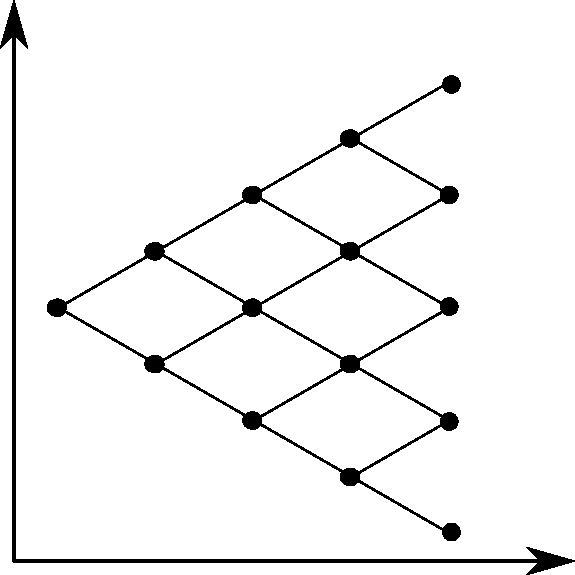
\includegraphics[scale=.5]{../plts/binomial-tree-example}
  \caption{Example of binomial tree}
  \label{fig:btex}
\end{figure}

Let $N$ be the depth of the binomial tree, i.e. the number of nodes from the
root to the last node. In the first place, the barrier is calculated by:
\begin{equation*}
  f_{N, j} = \max(S_{0}ujd(N - j) - K, 0)
\end{equation*}
with:
\begin{equation*}
  u = \expp{\sigma \sqrt{\Delta t}}, \quad d = \expp{-\sigma \sqrt{\Delta t}}, \quad
  p = \frac{\expp{r \Delta t} - d}{u - d}
\end{equation*}

Lastly, the tree is traversed backwards calculating each node by:
\begin{equation*}
  f_{i, j} = \expp{-r \Delta t} (p f_{i + 1, j+1} + (1 - p)  f_{i+1, j})
\end{equation*}

The pricing for the option is stored in the root of the tree, after completing
all calculations.

Three strikes where selected such that for each $K$ it happens that $S_0 > K$,
with $S_0 \approx 225$. The strikes with the comparison of the result of each
method is shown in Table \ref{tab:comp1}. For Monte Carlo, the selected
parameters were $M=3000$ and $W=500$. For finite differences, the selected
parameter was $NS = 1000$. Finally, for the binomial tree the selected parameter
was $N=100$.

\begin{table}[H]
\centering
\begin{tabular}{ccccc}
\hline
        & Black Scholes & Monte Carlo & Finite Diffs. & Binomial Tree \\
$K=200$ & 186.22        & 184.70      & 157.52        & 186.22        \\
$K=100$ & 205.65        & 204.29      & 191.91        & 205.65        \\
$K=50$  & 215.37        & 213.81      & 208.03        & 215.37        \\ \hline
\end{tabular}
\caption{Result for each method for two decimal places.}
\label{tab:comp1}
\end{table}

The method which was the closest one to the exact solution was the Binomial Tree
as the numbers are equal to two decimals. Then, it is followed by the Monte
Carlo simulation method, which was the second closest but the slowest algorithm.
Finally, the Finite Difference was the worst at estimating the pricing. In this
manner, by this small experiment, it can be stated that Binomial Tree is the
most precise and efficient method.

\subsection{Question 4}


\section{Sensitivity Analysis}

\subsection{Question 1}


\subsection{Question 2}


\subsection{Question 5}


\printbibliography
\end{document}
